\subsection{Sorting de arreglos}	
    \subsubsection{Conjuntos de numeros pseudoaleatorios utilizados para los experimentos}
    	Para este experimento se realizaron pruebas con diferentes longuitudes de arreglo, estas siempre
    	siendo una potencia de 2.\\
    	Las muestras de datos se generaron utilizando un generador de numeros pseudo-aleatorios
    	congruencial lineal con la misma semilla inicial.
        Asimismo luego de todos los ordenamientos de distinto tamaño de entrada y modo de procesamiento, se realiza una verificación de correctitud del algoritmo de ordenamiento para detectar posibles errores en el procesamiento o sincronización de los núcleos.
    \subsubsection{Implementación con un unico núcleo}
    	En este experimento se realiza un heap-sort sobre todos los arreglos de distinto tamaño.
    \subsubsection{Implementación con dos cores: Paralelización del algoritmo}
    	Se optó en este caso por un algoritmo propio que combinara varios ordenamientos conocidos con el objetivo de hacer mas facil la paralelización del experimento. En particular lo que se realiza es partir el arreglo en 2 mitades, donde cada core realiza heapsort sobre su mitad asignada y luego una intercalación de los resultados con un algoritmo tambien paralelo en el cual un core realiza el merge de los maximos y el otro el merge de los minimos, luego resta copiar los resultados y concluimos.

   	\begin{center}
        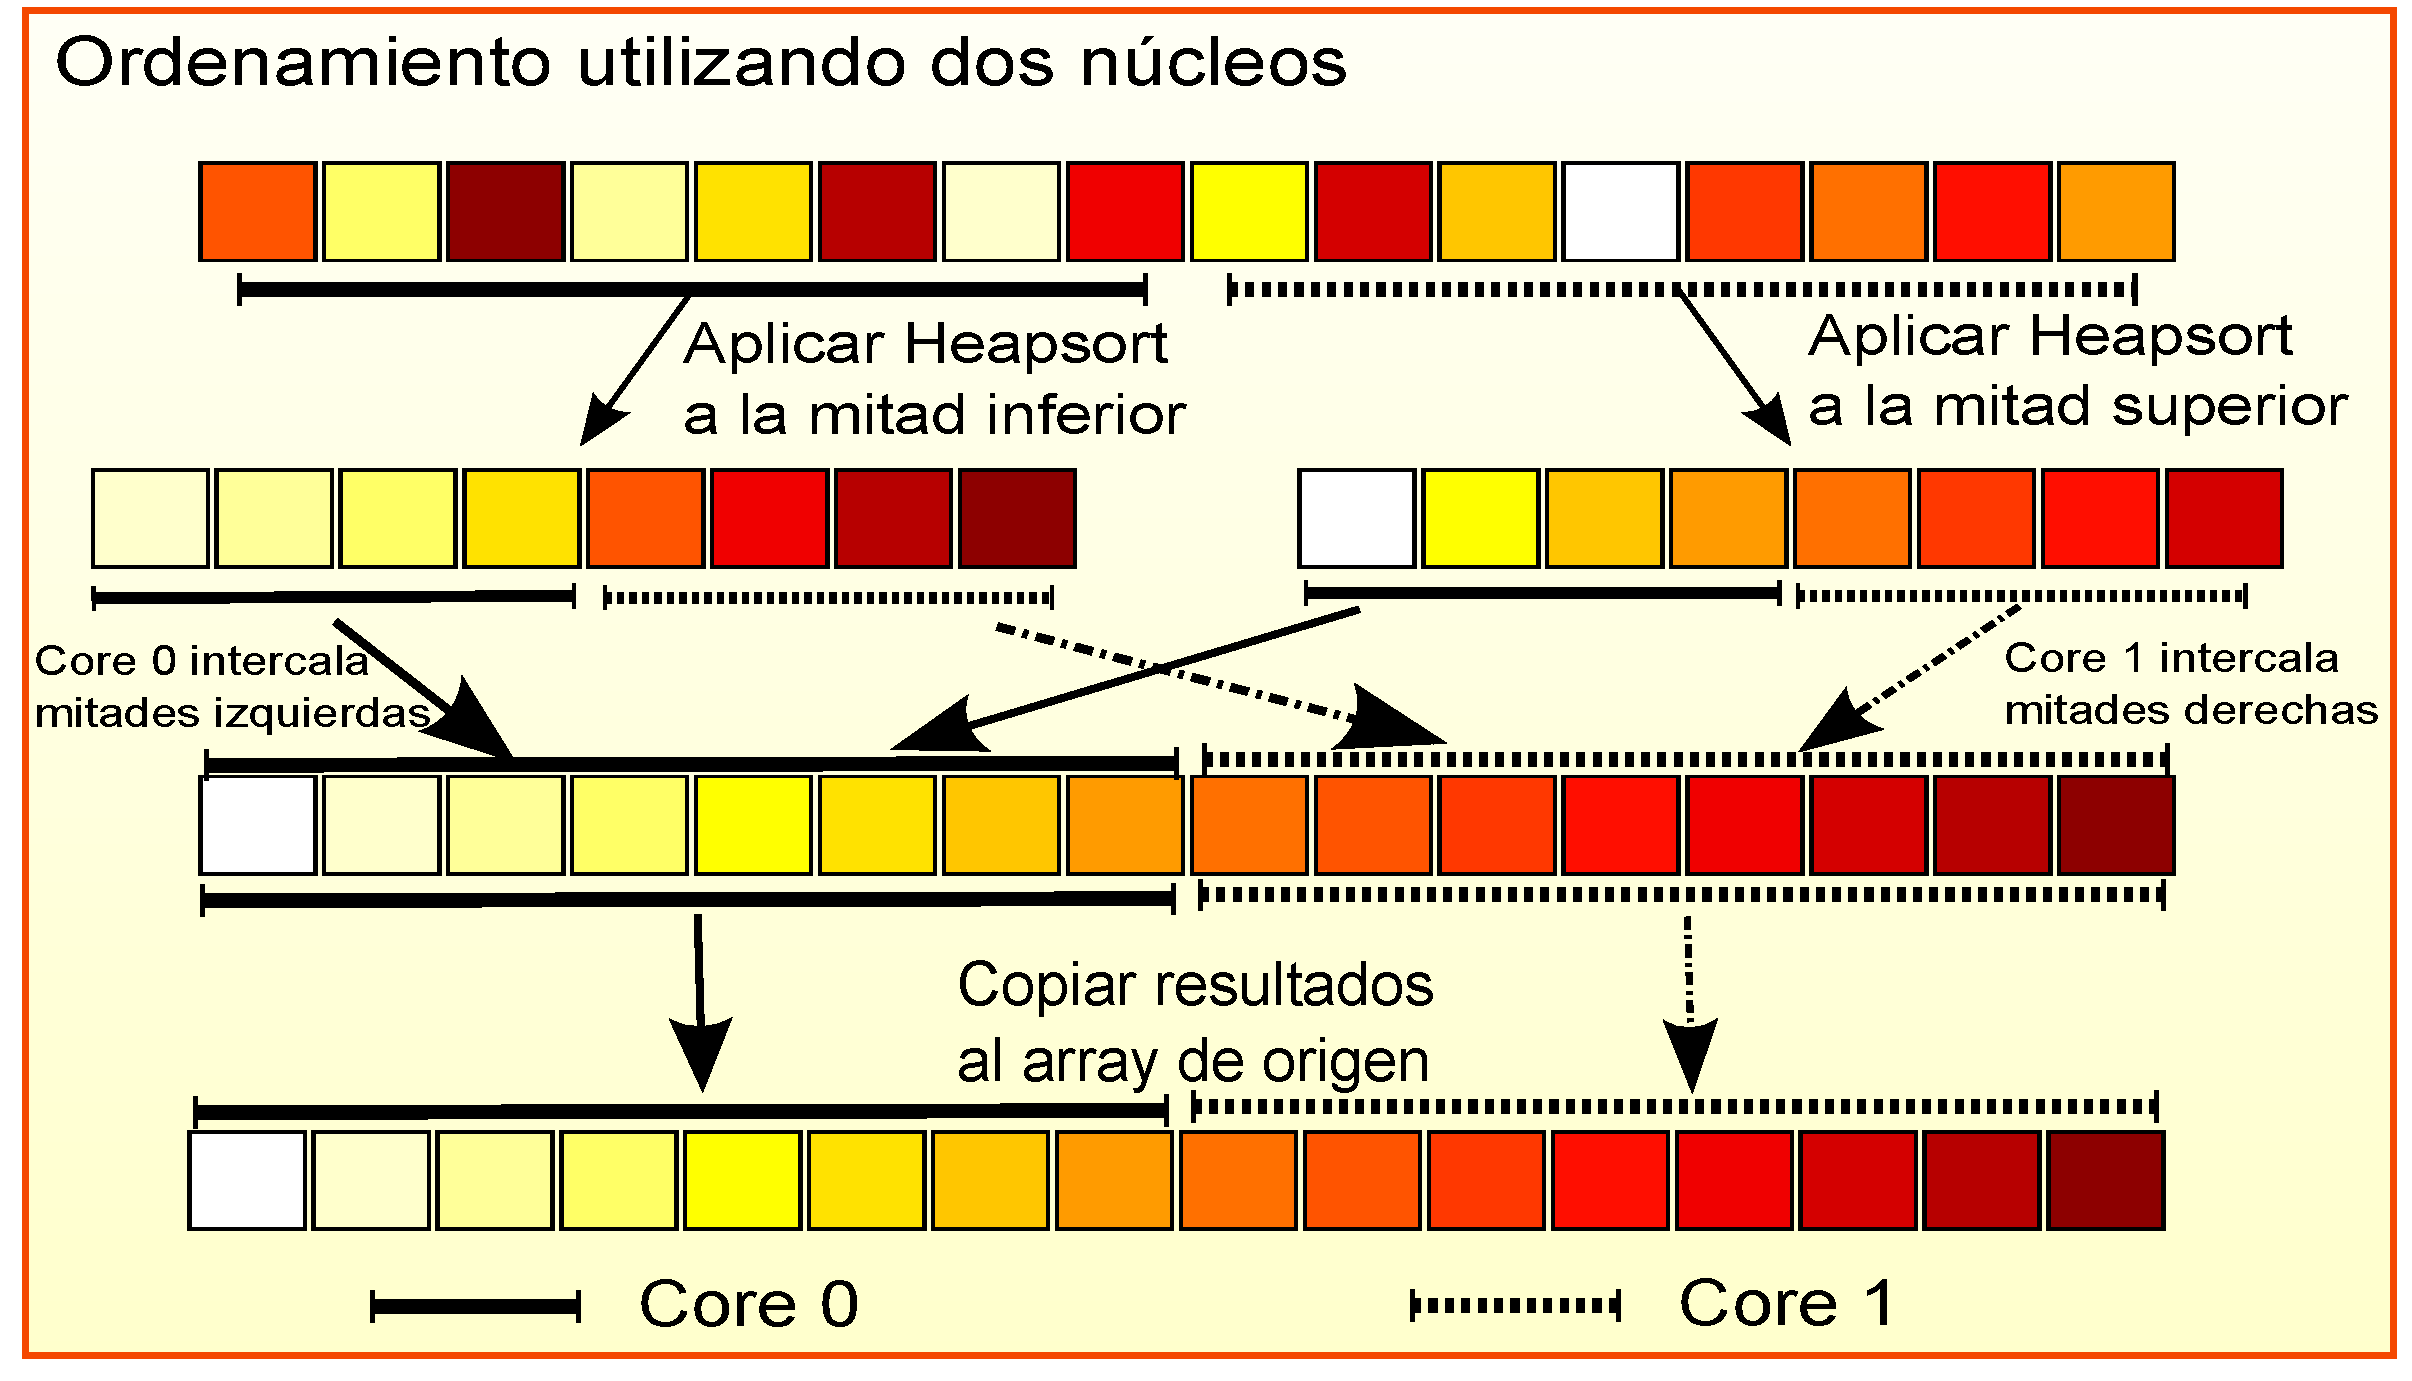
\includegraphics[height=9cm]{images/dualcore-sorting.pdf}
    \end{center}
    	

    \subsubsection{Implementación con dos cores: Sincronización con espera activa}
    	Para abordar el problema de la sincronización la primera implementacion fue basada en espera activa, en la que basicamente existen flags en los cuales los distintos núcleos indican su estado actual entre sí actualizando los diferentes flags, igualmente esto no es simétrico, hay 2 roles definidos, maestro y esclavo, el primero da las órdenes y espera la señal de finalización de las operaciones asignadas al núcleo esclavo.
    	El algoritmo funciona de la siguiente manera, siendo el bsp el master y el ap el slave:
    	\begin{enumerate}
    		\item Cuando el master empieza a ejecutar el algoritmo, el slave esta chequeando todo el tiempo una variable para ver si puede iniciar o no el trabajo.
    		
    		\item El master setea el flag de inicio del sort y empieza a ordenar su mitad del arreglo, mientras que el slave sale del loop de verificacion y empieza a ordenar su mitad del arreglo.
    		
    		\item Una vez que el master termina, se queda esperando a que el slave setee el flag de que termino la etapa en la que estaba. El slave cuando termina su etapa setea el flag que avisa que termino y se pone a chequear en un loop un flag para que le autorice a pasar a la siguiente etapa.

    		\item Cuando el master verifica que el slave termino, resetea los flags utilizados hasta ahora, y setea el flag de inicio de la etapa de merge, luego de lo cual se pone a realizar merge de su mitad. El slave, por su parte, una vez que verifica que puede pasar a la siguiente etapa, se pone hacer merge con su mitad, seteando un flag para avisar que termino.

    		\item El master, luego de verificar que el slave termino, setea el flag para iniciar la última etapa del algoritmo, que es la de copiar los resultados de los diferentes merge al arreglo original. Cada core por su lado copia los resultados de sus respectivos merge al array original. El slave cuando termina le avisa al master y se queda loopeando esperando la señal para arrancar el algoritmo de 0.

    		\item Una vez que el master verifico que el slave termino, resetea todos los flags utilizados hasta ahora, y sale de la función.

			\item Cuando se terminan todas las pruebas, se setea una variable global para avisarle al slave que puede salir de la función y pasar a modo de bajo consumo.
    	\end{enumerate}

   	\begin{center}
        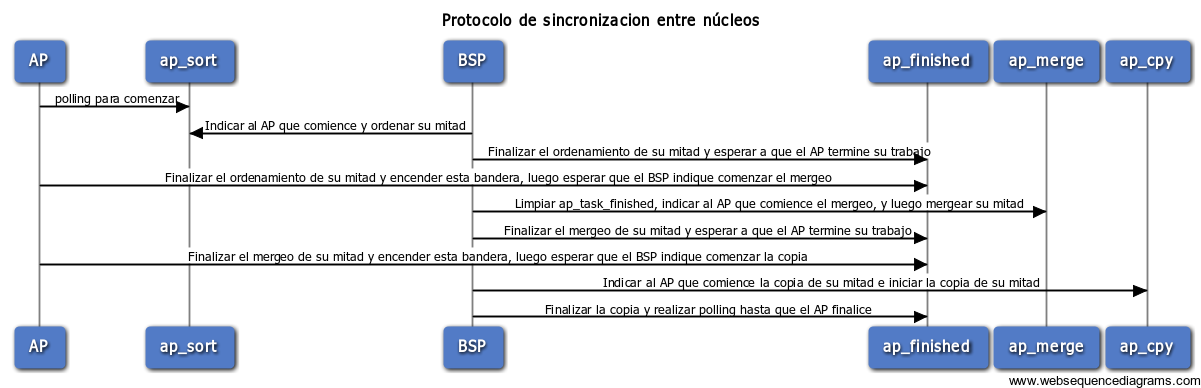
\includegraphics[height=5.5cm]{images/sync-sorting-seq.png}
    \end{center}

    \subsubsection{Implementación con dos cores: Sincronización con inter-processor interrupts}
    	En esta implementación, el slave se encuentra en modo de bajo consumo, y lo que hace el master es mandarle interrupciones específicas de acuerdo a la etapa en la que esta del algoritmo. En total son 3 interrupciones diferentes, las cuales hacen que el slave ordene, mergee y copie respectivamente.\\

    	En este caso el protocolo de sincronización para las tres etapas es:
    	\begin{enumerate}
    		\item El slave espera que el master envie una interrupcion para comenzar la etapa correspondiente.
    		\item El master realiza su trabajo asignado en dicha etapa, y al finalizar setea su registro RAX en cero y setea una variable bandera en 1 dando aviso de que finalizó y luego realiza polling al registro RAX mientras el valor sea cero.
    		\item El slave espera que el master finalice leyendo la variable bandera, esperando que su valor sea 1. Cuando esto ocurre, es enviada una interrupcion al master, y pasa a modo bajo consumo, es decir, se haltea.
    		\item El master recibe la interrupcion y en la ISR setea su registro RAX en 1, haciendo que salga del ciclo del item 2 para pasar a la siguiente etapa del algoritmo o finalizar segun corresponda.    		
    	\end{enumerate}


   	\begin{center}
        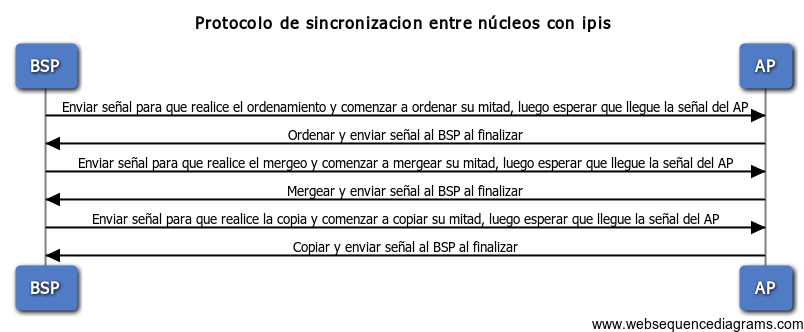
\includegraphics[height=6.5cm]{images/ipis-sorting-seq.png}
    \end{center}
